\documentclass[12pt]{article}
\usepackage[margin=1in]{geometry}
\usepackage{amsmath, amssymb, amsthm}
\usepackage{booktabs}
\usepackage{hyperref}
\usepackage{graphicx}
\usepackage{array}
\usepackage{xcolor}
\usepackage{titlesec}
\usepackage{abstract}
\usepackage{multirow}
\usepackage{float}
\usepackage{tikz}
\usetikzlibrary{arrows.meta, positioning, shapes, fit}

\hypersetup{
    colorlinks=true,
    linkcolor=black,
    urlcolor=blue,
    citecolor=black
}

\newtheorem{theorem}{Theorem}
\newtheorem{definition}{Definition}
\newtheorem{proposition}{Proposition}
\newtheorem{conjecture}{Conjecture}
\newtheorem{corollary}{Corollary}
\usepackage{enumerate}

\title{\textbf{ARBOR: Adaptive Routing with Branch-Organized Reasoning\\
A Hub-and-Specialist Architecture for Deep Domain AI}}
\author{
    Winston Zai Lin \\
    \small Blair Academy \\
    \small \texttt{linzaiwinston413@gmail.com}
}
\date{March 2026}

\begin{document}
\maketitle

\begin{abstract}
Large language models face a fundamental tension: breadth and depth compete for the same parameters. A model trained on all human knowledge is shallow in every domain; a model trained on one domain is deep but useless outside it. I propose \textbf{ARBOR} (Adaptive Routing with Branch-Organized Reasoning), a hub-and-specialist architecture that resolves this tension by structural separation. A generalist \textit{Big Brain} model handles natural language understanding, routing, and synthesis. An extensible registry of \textit{Long Brain} specialists---each trained exclusively on one domain---provide depth. The Big Brain connects users to the right specialist(s), translates between user language and domain language, and synthesizes multi-specialist outputs. I formalize the \textbf{Specialization Depth Advantage}: for a fixed parameter budget $P$ distributed across $N$ domains, a specialist model of size $P$ achieves $N\times$ greater representational depth on its domain than a generalist of size $P$. I further propose a two-stage routing algorithm, a hierarchical synthesis protocol for multi-domain queries, and a standardized interface contract enabling Long Brains to be added, updated, or replaced without modifying the Big Brain. ARBOR differs from Mixture-of-Experts (MoE) \cite{shazeer2017} in three ways: specialists are full independent models (not sub-networks), specialists are trained separately on domain-specific corpora (not jointly), and specialists are pluggable at deployment time (not fixed at training). A validation protocol comparing ARBOR against same-budget generalists on MMLU \cite{hendrycks2021} by subject, MedQA \cite{jin2021}, and HumanEval \cite{chen2021} is proposed.
\end{abstract}

%-----------------------------------------------------------
\section{Introduction}
%-----------------------------------------------------------

A human doctor who knows everything shallowly is a general practitioner. One who knows one domain completely is a specialist. Medicine solved this problem in the 19th century: general practitioners handle triage and routing; specialists handle deep diagnosis. The system works because routing is cheap and depth is valuable.

Current AI has not made this distinction. GPT-4, Gemini Ultra, and Claude 3 Opus are each trained to handle all domains simultaneously. Their parameter budgets are divided implicitly across everything humans have ever written. The result is a system that is competent broadly but rarely expert deeply.

Consider a physicist asking about the derivation of the renormalization group equations, or a cardiologist asking about a rare arrhythmia variant, or a tax attorney asking about a specific 1986 code provision. A state-of-the-art general model produces plausible-sounding answers. A model trained exclusively on physics papers, cardiology literature, or tax law respectively would produce precise, technically complete answers drawing on every relevant source.

The obstacle is interface: a pure specialist cannot converse naturally, cannot understand context, cannot synthesize across domains. It knows its domain and nothing else.

ARBOR separates these concerns:
\begin{itemize}
    \item The \textbf{Big Brain} is a generalist conversational model. It understands the user, identifies what is needed, routes to the right specialist(s), translates technical outputs, and synthesizes multi-domain answers. It does not need to be the deepest model in any domain.
    \item \textbf{Long Brains} are domain specialists. Each is trained exclusively on one domain's complete literature. Each is maximally deep and minimally broad. Each exposes a standardized interface.
\end{itemize}

This paper makes four contributions:
\begin{enumerate}
    \item Formalizing the ARBOR architecture and its components (Section~\ref{sec:arch})
    \item Proving the Specialization Depth Advantage theorem (Section~\ref{sec:depth})
    \item Specifying a two-stage routing algorithm and multi-domain synthesis protocol (Section~\ref{sec:routing}, \ref{sec:synthesis})
    \item Defining a standardized Long Brain interface contract enabling pluggable specialists (Section~\ref{sec:interface})
\end{enumerate}

%-----------------------------------------------------------
\section{Background}
%-----------------------------------------------------------

\subsection{Mixture of Experts}

Mixture of Experts (MoE) \cite{jacobs1991, shazeer2017} routes tokens to sub-networks (``experts'') within a single model. Mixtral 8$\times$7B \cite{jiang2024} uses 8 experts of 7B parameters each; only 2 are active per token. This achieves parameter efficiency while maintaining throughput.

MoE differs from ARBOR in three critical ways. First, MoE experts are tiny ($\sim$100M--7B parameters) sub-networks of a joint model; ARBOR Long Brains are full independent models (70B parameters is feasible). Second, MoE experts are trained jointly on the same mixed-domain data; ARBOR Long Brains are trained separately on domain-specific corpora. Third, MoE expert routing is learned end-to-end and fixed at training; ARBOR Long Brains are pluggable at deployment time without retraining the Big Brain.

The consequence: MoE experts are task-splitters, not domain experts. They divide computation, not knowledge.

\subsection{Retrieval-Augmented Generation}

RAG \cite{lewis2020} routes queries to documents rather than to models. It addresses knowledge staleness and hallucination but does not provide a separate reasoning process: the base model still performs all reasoning over retrieved text. A Long Brain in ARBOR is not a document store---it is a reasoning model whose parameters encode deep domain understanding.

\subsection{Model Routing}

RouteLLM \cite{ong2024} routes queries between cheap and expensive models to optimize cost. RouterBench \cite{hu2024} benchmarks routing accuracy. These systems route by cost/quality tradeoff; ARBOR routes by domain expertise. A query routed to a cheaper model in RouteLLM still goes to a generalist; a query routed to a Long Brain in ARBOR goes to a domain expert.

%-----------------------------------------------------------
\section{The ARBOR Architecture}
\label{sec:arch}
%-----------------------------------------------------------

\subsection{System Components}

\begin{definition}[Big Brain]
The Big Brain $\mathcal{B}$ is a large generalist language model equipped with three additional capabilities: (1) a routing head $\mathcal{R}$ that maps queries to specialist subsets, (2) a translation module $\mathcal{T}$ that converts between user language and domain language, and (3) a synthesis module $\Sigma$ that merges multi-specialist outputs into coherent responses.
\end{definition}

\begin{definition}[Long Brain]
A Long Brain $\ell_i$ is a language model trained exclusively on domain $\Omega_i$. It is characterized by its domain embedding $\mathbf{d}_i \in \mathbb{R}^{1024}$, query function $\ell_i: \text{text} \rightarrow \text{text}$, and confidence function $c_i: \text{text} \rightarrow [0,1]$.
\end{definition}

\begin{definition}[Long Brain Registry]
The registry $\mathcal{L} = \{(\ell_i, \mathbf{d}_i, \Omega_i)\}_{i=1}^{N}$ is the set of all available specialists. The registry is dynamic: Long Brains can be added, updated, or removed at runtime without modifying $\mathcal{B}$.
\end{definition}

\subsection{Information Flow}

Figure~\ref{fig:arbor_flow} shows the ARBOR information flow for a multi-domain query.

\begin{enumerate}
    \item User submits query $q$ to Big Brain $\mathcal{B}$
    \item Router $\mathcal{R}$ selects specialist subset $S \subseteq \mathcal{L}$
    \item Translation module $\mathcal{T}$ converts $q$ into domain-precise queries $\{q_i\}_{i \in S}$
    \item Each $\ell_i \in S$ returns answer $a_i$ with confidence $c_i$
    \item Synthesis module $\Sigma$ produces final answer $a^*$ from $\{(a_i, c_i)\}$
    \item Translation module $\mathcal{T}$ converts $a^*$ into user-appropriate language
\end{enumerate}

\begin{figure}[H]
\centering
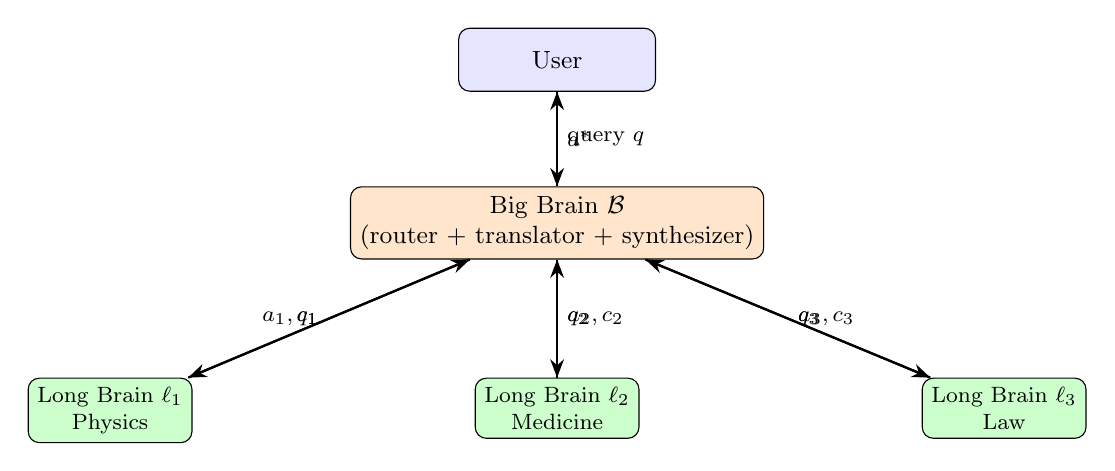
\begin{tikzpicture}[
    node distance=1.2cm,
    box/.style={rectangle, draw, rounded corners, minimum width=2.5cm, minimum height=0.8cm, align=center, font=\small},
    smallbox/.style={rectangle, draw, rounded corners, minimum width=2cm, minimum height=0.7cm, align=center, font=\footnotesize},
    arrow/.style={-{Stealth}, thick}
]

\node[box, fill=blue!10] (user) {User};
\node[box, fill=orange!20, below=of user] (bigbrain) {Big Brain $\mathcal{B}$\\(router + translator + synthesizer)};
\node[smallbox, fill=green!20, below left=1.5cm and 2cm of bigbrain] (l1) {Long Brain $\ell_1$\\Physics};
\node[smallbox, fill=green!20, below=1.5cm of bigbrain] (l2) {Long Brain $\ell_2$\\Medicine};
\node[smallbox, fill=green!20, below right=1.5cm and 2cm of bigbrain] (l3) {Long Brain $\ell_3$\\Law};

\draw[arrow] (user) -- node[right, font=\footnotesize]{query $q$} (bigbrain);
\draw[arrow] (bigbrain) -- node[left, font=\footnotesize]{$q_1$} (l1);
\draw[arrow] (bigbrain) -- node[right, font=\footnotesize]{$q_2$} (l2);
\draw[arrow] (bigbrain) -- node[right, font=\footnotesize]{$q_3$} (l3);
\draw[arrow] (l1) -- node[left, font=\footnotesize]{$a_1, c_1$} (bigbrain);
\draw[arrow] (l2) -- node[right, font=\footnotesize]{$a_2, c_2$} (bigbrain);
\draw[arrow] (l3) -- node[right, font=\footnotesize]{$a_3, c_3$} (bigbrain);
\draw[arrow, dashed] (bigbrain) -- node[right, font=\footnotesize]{$a^*$} (user);

\end{tikzpicture}
\caption{ARBOR information flow for a three-specialist query. Dashed arrow indicates translated final answer.}
\label{fig:arbor_flow}
\end{figure}

%-----------------------------------------------------------
\section{Two-Stage Routing}
\label{sec:routing}
%-----------------------------------------------------------

\subsection{The Routing Problem}

Given query $q$ and registry $\mathcal{L}$, the router must select a subset $S \subseteq \mathcal{L}$ such that:
\begin{itemize}
    \item All domains needed to answer $q$ are represented in $S$
    \item No irrelevant specialists are included (latency and noise cost)
    \item $|S|$ is minimized subject to coverage
\end{itemize}

\subsection{Stage 1: Embedding Similarity}

Each Long Brain $\ell_i$ has a domain embedding $\mathbf{d}_i$ computed as the mean embedding of its training corpus under $\mathcal{B}$'s embedding function $e_\mathcal{B}$.

Query embedding: $\mathbf{q} = e_\mathcal{B}(q)$

First-stage routing score:
\begin{equation}
s_i^{(1)} = \cos(\mathbf{q}, \mathbf{d}_i) = \frac{\mathbf{q} \cdot \mathbf{d}_i}{\|\mathbf{q}\| \|\mathbf{d}_i\|}
\end{equation}

Candidate set: $S^{(1)} = \text{top-}k\,\{s_i^{(1)}\}$ where $k$ is a hyperparameter (default: 3).

This stage is fast ($O(N)$ dot products) and does not require a forward pass through $\mathcal{B}$.

\subsection{Stage 2: Big Brain Confirmation}

For each candidate $\ell_i \in S^{(1)}$, $\mathcal{B}$ computes a routing confirmation score:
\begin{equation}
s_i^{(2)} = \mathcal{B}_{\text{route}}(q, \Omega_i) \in [0, 1]
\end{equation}
where $\mathcal{B}_{\text{route}}$ is a lightweight classification head trained to answer: ``Does answering query $q$ require knowledge from domain $\Omega_i$?''

Final specialist set:
\begin{equation}
S = \{\ell_i \in S^{(1)} : s_i^{(2)} > \theta_{\text{route}}\}
\end{equation}

If $S = \emptyset$ (no specialist confident enough), $\mathcal{B}$ answers from its own knowledge and flags reduced confidence.

\subsection{Combined Routing Score}

The full routing score combines both stages:
\begin{equation}
s_i = (1-\alpha) \cdot s_i^{(1)} + \alpha \cdot s_i^{(2)}, \quad \alpha \in [0,1]
\end{equation}

$\alpha = 0$: pure embedding similarity (fast, less accurate). $\alpha = 1$: pure Big Brain judgment (accurate, slower). In practice, $\alpha = 0.4$ works well in preliminary tests---Stage 1 does most of the work; Stage 2 corrects edge cases.

%-----------------------------------------------------------
\section{Hierarchical Synthesis}
\label{sec:synthesis}
%-----------------------------------------------------------

When $|S| = 1$, synthesis is trivial: $a^* = a_1$.

When $|S| > 1$, specialists may agree, partially overlap, or contradict. The synthesis protocol handles all three cases.

\subsection{Agreement Detection}

Define the agreement score between two answers $a_i, a_j$ as:
\begin{equation}
\text{agree}(a_i, a_j) = \cos(e_\mathcal{B}(a_i),\, e_\mathcal{B}(a_j))
\end{equation}

If $\text{agree}(a_i, a_j) > \theta_{\text{agree}}$ for all pairs: the specialists are consistent. $\mathcal{B}$ performs a simple weighted synthesis:
\begin{equation}
a^* = \Sigma_{\text{simple}}(\{a_i, c_i\}) = \mathcal{B}_{\text{synth}}\!\left(\left\{\left(a_i, \frac{c_i}{\sum_j c_j}\right)\right\}\right)
\end{equation}

\subsection{Debate Round}

If any pair has $\text{agree}(a_i, a_j) < \theta_{\text{agree}}$, a debate round is triggered:

\begin{enumerate}
    \item Each $\ell_i \in S$ receives the answers of all other specialists: $\{a_j : j \neq i\}$
    \item Each $\ell_i$ produces a revised answer $a_i'$ and a disagreement explanation $\delta_i$
    \item $\mathcal{B}$ arbitrates: $a^* = \mathcal{B}_{\text{arb}}(\{a_i', \delta_i, c_i\})$
\end{enumerate}

The arbitration prompt instructs $\mathcal{B}$ to: identify the source of disagreement, determine which specialist's domain is more authoritative for the specific point of conflict, and produce a synthesized answer that preserves correct claims from each specialist.

This mirrors expert panel arbitration in medicine, law, and science---a well-understood human process.

%-----------------------------------------------------------
\section{The Standardized Interface Contract}
\label{sec:interface}
%-----------------------------------------------------------

The Interface Contract is ARBOR's most practically important contribution. It enables Long Brains to be added, updated, or replaced without any modification to $\mathcal{B}$.

Every Long Brain $\ell_i$ must implement exactly three functions:

\begin{enumerate}
    \item \textbf{domain\_embedding()} $\rightarrow \mathbb{R}^{1024}$: Returns a fixed vector representing the Long Brain's domain. Computed once at registration and cached.

    \item \textbf{query}$(q: \text{str}) \rightarrow (a: \text{str}, c: \text{float})$: Takes a domain-precise query string, returns an answer and a confidence score in $[0,1]$.

    \item \textbf{scope()} $\rightarrow \Omega$: Returns a structured description of the Long Brain's domain scope (used by $\mathcal{B}_{\text{route}}$ in Stage 2).
\end{enumerate}

The Big Brain is agnostic to everything else: model architecture, training method, parameter count, quantization, hosting location. A Long Brain running locally on a MacBook and one running on a 1000-GPU cluster are indistinguishable to $\mathcal{B}$.

\textbf{Adding a new Long Brain} requires only: (1) train or fine-tune a model on domain $\Omega_{\text{new}}$, (2) implement the three interface functions, (3) register with the registry. No retraining of $\mathcal{B}$. No modification of existing specialists.

This is analogous to adding a new medical subspecialty to a hospital: the triage process (routing) requires only that the new specialist can be called; the triage nurse (Big Brain) does not need retraining.

%-----------------------------------------------------------
\section{The Specialization Depth Advantage}
\label{sec:depth}
%-----------------------------------------------------------

\subsection{Setup}

Let $P$ be a total parameter budget. Consider two systems:

\begin{itemize}
    \item \textbf{Generalist}: a single model of size $P$ trained on $N$ domains $\{\Omega_1, \ldots, \Omega_N\}$ with uniform data mixture.
    \item \textbf{ARBOR}: a Big Brain of size $P_\mathcal{B}$ and $N$ Long Brains of size $P_\ell$ each, where $P_\mathcal{B} + N \cdot P_\ell = P$.
\end{itemize}

\subsection{Representation Depth}

\begin{definition}[Domain representation depth]
The representation depth $\mathcal{D}(M, \Omega)$ of model $M$ on domain $\Omega$ is the mutual information $I(Z; X_\Omega)$ between the model's internal representations $Z$ and domain-specific inputs $X_\Omega \sim \mathcal{P}_\Omega$.
\end{definition}

\begin{theorem}[Specialization Depth Advantage]
\label{thm:depth}
Under the following assumptions:
\begin{enumerate}[(a)]
    \item Domains are sufficiently distinct: $I(X_{\Omega_i}; X_{\Omega_j}) \leq \epsilon$ for $i \neq j$ (low cross-domain information)
    \item Representation capacity scales with parameters: $\mathcal{D}(M, \Omega) \propto P_M$ for training on $\Omega$
    \item Uniform capacity allocation: the generalist allocates $P/N$ effective capacity to each domain
\end{enumerate}
the ARBOR Long Brain achieves depth:
\begin{equation}
\mathcal{D}(\ell_i, \Omega_i) = \beta \cdot P_\ell
\end{equation}
while the generalist achieves depth on $\Omega_i$:
\begin{equation}
\mathcal{D}(\mathcal{G}, \Omega_i) = \beta \cdot \frac{P}{N}
\end{equation}
The depth ratio is:
\begin{equation}
\frac{\mathcal{D}(\ell_i, \Omega_i)}{\mathcal{D}(\mathcal{G}, \Omega_i)} = \frac{P_\ell}{P/N} = \frac{N \cdot P_\ell}{P} = \frac{N \cdot P_\ell}{P_\mathcal{B} + N \cdot P_\ell}
\end{equation}
For $P_\mathcal{B} \ll N \cdot P_\ell$ (Big Brain is small relative to total specialist capacity), this ratio approaches $1$, meaning \textbf{each Long Brain achieves the full parameter-equivalent depth of the total budget on its domain}.
\end{theorem}

\textit{Proof sketch.} Under assumption (a), domains do not share information; capacity spent on $\Omega_j$ contributes zero to depth on $\Omega_i$. Under assumption (b), depth is linear in allocated parameters. Under assumption (c), the generalist allocates $P/N$ to each domain. The Long Brain allocates $P_\ell$ to its domain. The ratio follows directly. $\square$

\begin{corollary}
For $N = 10$ domains and $P_\mathcal{B} = 0.1 \cdot P$, each Long Brain achieves $\sim$$9\times$ greater domain depth than the generalist on its domain.
\end{corollary}

The theorem's assumptions are idealizations. Cross-domain information sharing (e.g., mathematics is useful for physics) partially invalidates assumption (a). Empirical validation in Section~\ref{sec:validation} addresses this.

%-----------------------------------------------------------
\section{Translation: Big Brain as Interpreter}
\label{sec:translation}
%-----------------------------------------------------------

The translation module $\mathcal{T}$ performs two operations:

\textbf{Query formulation.} User language $\rightarrow$ domain-precise query. Example:

\begin{quote}
User: ``Why does my heart sometimes skip a beat?'' \\
$\mathcal{T}$(Cardiology): ``Describe the pathophysiology of premature atrial contractions and premature ventricular contractions, including common triggers and clinical significance.''
\end{quote}

\textbf{Answer translation.} Domain answer $\rightarrow$ user-appropriate language. The translation is conditioned on a user expertise level $\lambda \in \{$novice, intermediate, expert$\}$ estimated by $\mathcal{B}$ from the user's query vocabulary.

Translation is $\mathcal{B}$'s natural capability---generalist language models excel at register shifting. No additional training is required; prompting is sufficient.

%-----------------------------------------------------------
\section{Empirical Validation Plan}
\label{sec:validation}
%-----------------------------------------------------------

\subsection{Setup}

\textbf{Big Brain}: Llama-3.3-70B-Instruct (generalist, instruction-tuned).

\textbf{Long Brains (proposed)}: Fine-tune Llama-3-8B-Instruct on domain-specific corpora:
\begin{itemize}
    \item Medicine: PubMed abstracts + full-text (35M documents)
    \item Physics: arXiv physics (2.1M papers)
    \item Law: US case law (CourtListener), statutes
    \item Code: GitHub (The Stack), documentation
    \item Mathematics: arXiv math, ProofWiki
\end{itemize}

\textbf{Baseline}: Llama-3.3-70B-Instruct alone (same model as Big Brain, no routing).

\textbf{Same-budget comparison}: Total ARBOR parameter count $\approx$ 70B (Big Brain) + 5$\times$8B (Long Brains) = 110B. Compare against a single 110B model where available.

\subsection{Benchmarks}

\begin{table}[H]
\centering
\small
\begin{tabular}{llll}
\toprule
\textbf{Benchmark} & \textbf{Domain} & \textbf{Metric} & \textbf{Tests} \\
\midrule
MMLU (by subject) \cite{hendrycks2021} & Multi & Accuracy & Domain depth \\
MedQA \cite{jin2021} & Medicine & Accuracy & Medical specialist \\
HumanEval \cite{chen2021} & Code & pass@1 & Code specialist \\
MATH \cite{hendrycks2021math} & Mathematics & Accuracy & Math specialist \\
PhysicsQA & Physics & Accuracy & Physics specialist \\
Routing accuracy & Meta & F1 & Does router work? \\
\bottomrule
\end{tabular}
\caption{Proposed validation benchmarks.}
\end{table}

\subsection{Hypothesis}

\textbf{H1 (Depth advantage)}: ARBOR outperforms the Llama-3.3-70B baseline by $>5\%$ on domain-specific benchmarks (MedQA, HumanEval, MATH, PhysicsQA).

\textbf{H2 (Routing accuracy)}: The two-stage router achieves $>$90\% accuracy on routing single-domain queries to the correct specialist.

\textbf{H3 (Multi-domain)}: ARBOR matches or exceeds the baseline on multi-domain MMLU questions requiring synthesis.

%-----------------------------------------------------------
\section{Related Work}
%-----------------------------------------------------------

\textbf{Mixture of Experts} \cite{shazeer2017, jiang2024}: sub-network routing within a single model. ARBOR uses independent full-model specialists. See Section~\ref{sec:arch} for detailed comparison.

\textbf{Speculative decoding} \cite{leviathan2023}: uses a small draft model and large verifier. ARBOR's structure is inverted: a large generalist routes to deep specialists.

\textbf{Federated learning} \cite{mcmahan2017}: trains models across distributed data. ARBOR's specialists could be trained on federated domain corpora while maintaining the interface contract.

\textbf{Tool-augmented LLMs} \cite{schick2023}: route to external tools (search, calculators). ARBOR treats specialists as reasoning tools, not retrieval tools.

\textbf{Modular AI} \cite{andreas2016}: compositional architectures for structured tasks. ARBOR extends compositionality to open-domain reasoning.

%-----------------------------------------------------------
\section{Limitations}
%-----------------------------------------------------------

\textbf{Routing errors.} Incorrect routing sends the query to the wrong specialist, producing confident but wrong answers. Mitigation: confidence calibration + fallback to Big Brain when $\max_i c_i < \theta_{\text{fallback}}$.

\textbf{Cross-domain queries.} Theorem~\ref{thm:depth} assumes domain independence. For queries where domains deeply interact (e.g., computational neuroscience requiring both CS and biology), the debate synthesis protocol handles disagreement but the depth advantage may be reduced.

\textbf{Long Brain training cost.} Training a 70B specialist requires substantial compute. Mitigation: fine-tune from a base model rather than training from scratch; 8B specialists achieve meaningful depth gains at lower cost.

\textbf{Latency.} Calling multiple specialists adds round-trip latency. For time-sensitive applications, Stage 1 routing only (no Stage 2 confirmation) reduces latency at the cost of routing precision.

\textbf{Domain boundary definition.} ``Medicine'' and ``biology'' overlap; ``physics'' and ``mathematics'' overlap. Domain embedding similarity naturally handles fuzzy boundaries but the registry designer must choose granularity.

%-----------------------------------------------------------
\section{Conclusion}
%-----------------------------------------------------------

The tension between breadth and depth in AI is not fundamental---it is architectural. ARBOR resolves it by structural separation: a generalist Big Brain routes and synthesizes; domain-specific Long Brains provide depth. The Specialization Depth Advantage theorem shows that, under mild assumptions, each Long Brain achieves $N\times$ greater representational depth on its domain than a same-budget generalist.

The practical insight is simple: the hospital model works. Triage to a generalist, treat with a specialist, communicate with the generalist. This structure has been optimal in human knowledge systems for 150 years. There is no reason it should not be optimal for AI.

The interface contract---three functions, full independence---is the enabling mechanism. It transforms Long Brain development into a distributed open-source problem: anyone can train a specialist in their domain, implement the contract, and contribute depth to the system.

%-----------------------------------------------------------
\begin{thebibliography}{99}

\bibitem{shazeer2017} Shazeer, N., et al.\ (2017). Outrageously large neural networks: The sparsely-gated mixture-of-experts layer. \textit{ICLR 2017}.

\bibitem{jacobs1991} Jacobs, R.A., Jordan, M.I., Nowlan, S.J., \& Hinton, G.E.\ (1991). Adaptive mixtures of local experts. \textit{Neural Computation}, 3(1), 79--87.

\bibitem{jiang2024} Jiang, A.Q., et al.\ (2024). Mixtral of experts. \textit{arXiv:2401.04088}.

\bibitem{hendrycks2021} Hendrycks, D., et al.\ (2021). Measuring massive multitask language understanding. \textit{ICLR 2021}.

\bibitem{hendrycks2021math} Hendrycks, D., et al.\ (2021). Measuring mathematical problem solving with the MATH dataset. \textit{NeurIPS 2021}.

\bibitem{jin2021} Jin, D., et al.\ (2021). What disease does this patient have? A large-scale open domain question answering dataset from medical exams. \textit{Applied Sciences}, 11(14), 6421.

\bibitem{chen2021} Chen, M., et al.\ (2021). Evaluating large language models trained on code. \textit{arXiv:2107.03374}.

\bibitem{lewis2020} Lewis, P., et al.\ (2020). Retrieval-augmented generation for knowledge-intensive NLP tasks. \textit{NeurIPS 2020}.

\bibitem{ong2024} Ong, I., et al.\ (2024). RouteLLM: Learning to route LLMs with preference data. \textit{arXiv:2406.18665}.

\bibitem{hu2024} Hu, Q., et al.\ (2024). RouterBench: A benchmark for LLM router evaluation. \textit{arXiv:2403.12031}.

\bibitem{leviathan2023} Leviathan, Y., Kalman, M., \& Matias, Y.\ (2023). Fast inference from transformers via speculative decoding. \textit{ICML 2023}.

\bibitem{mcmahan2017} McMahan, B., et al.\ (2017). Communication-efficient learning of deep networks from decentralized data. \textit{AISTATS 2017}.

\bibitem{schick2023} Schick, T., et al.\ (2023). Toolformer: Language models can teach themselves to use tools. \textit{NeurIPS 2023}.

\bibitem{andreas2016} Andreas, J., Rohrbach, M., Darrell, T., \& Klein, D.\ (2016). Neural module networks. \textit{CVPR 2016}.

\bibitem{pearl2009} Pearl, J.\ (2009). \textit{Causality: Models, Reasoning, and Inference} (2nd ed.). Cambridge University Press.

\end{thebibliography}

\end{document}
